\documentclass[11pt]{article}
\usepackage{sectsty}
\usepackage{graphicx}
\usepackage[T1]{fontenc}
\usepackage{multicol}
\usepackage{hyperref}
\usepackage{float}
% Margins
\topmargin=-0.5in
\evensidemargin=0in
\oddsidemargin=0in
\textwidth=6.5in
\textheight=9.0in
\headsep=0.25in

\title{ Przewidywanie liczby ludności w Polsce za pomocą modeli regresji liniowej na podstawie zmiennych demograficznych}
\author{ Krzysztof Kulka
        \\ 272667@student.pwr.edu.pl \\ MSiD Lab Wtorek 9.15 NP }
\date{\today}

\renewcommand{\contentsname}{Spis treści}
\begin{document}
\maketitle	
\pagebreak

\setcounter{tocdepth}{4}
\setcounter{secnumdepth}{4}
\tableofcontents
 \pagebreak


\section{Wstęp}
Problemem projektu jest analiza możliwości modelów regresji liniowej do przewidywania liczby ludności w Polsce. W tym celu wykorzystane zostaną dane historyczne dotyczące demografi, oraz innych czynników wpływających na liczebność populacji.
Przedstawiona analiza ma na celu rozstrzygnięcie czy model regresji liniowej jest odpowiedni do przewidywania liczby ludności w Polsce, oraz jakie modele sprawdzają się do tego najlepiej.
Analizie zostaną poddane następujące czynniki:
\begin{itemize}
\item Historyczna liczba ludności
\item Imigracja do kraju
\item Wskaźnik dzietności
\item Oczekiwana długość życia
\item Urbanizacja
\item Wskaźnik zmiany populacji na przestrzeni ostatnich 5 lat
\end{itemize}
Zbadane zaś zostaną następujące modele regresji:
\begin{itemize}
\item Regresja liniowa
\item Regresja typu Ridge
\item Regresja Lasso
\item Regresja Elastic Net
\item Regresja Bayesian Ridge
\end{itemize}
\section{Zbiór danych i jego analiza}
\subsection{Opis zbioru danych}
Zbiór danych zawiera informacje na temat historycznej liczby ludności, imigracji do kraju, wskazniku dzietnosci, oczekiwanej
długości życia w momencie urodzenia na przestrzeni lat 1960-2023.
Dane zostały pobrane z serwisu internetowego World Bank\cite{wbd} Dane dotyczą około 260 krajów. 
Dodatkowo informacje na temat urbanizacji
zostały pobrane z serwisu internetowego Zintegrowana Platforma Edukacyjna Ministerstwa Edukacji Narodowej\cite{zpe}, a wskaźnik zmiany populacji na przestrzeni ostatnich 5 lat został obliczony na podstawie danych historycznych.
\subsection{Przykładowe dane}
\begin{table}[!ht]
        \centering
        \resizebox{\textwidth}{!}{\begin{tabular}{|l|l|l|l|l|l|l|}
        \hline
            "Country Name" & "Country Code" & "Indicator Name" & "Indicator Code" & "1960" & "1961" & ... \\ \hline
            "Aruba" & "ABW" & "Fertility rate, total (births per woman)" & "SP.DYN.TFRT.IN" & "4.82" & "4.655" & ... \\ \hline
            "Africa Eastern and Southern" & "AFE" & "Fertility rate, total (births per woman)" & "SP.DYN.TFRT.IN" & "6.72412501084242" & "6.74275210020318" & ...\\ \hline
            "Afghanistan" & "AFG" & "Fertility rate, total (births per woman)" & "SP.DYN.TFRT.IN" & "7.282" & "7.284" & ... \\ \hline
            "Africa Western and Central" & "AFW" & "Fertility rate, total (births per woman)" & "SP.DYN.TFRT.IN" & "6.45844789624312" & "6.47151755185967" & ... \\ \hline
                ... \\
        \end{tabular}}
        \caption{Wycinek danych z zbioru dzietności na kobietę}
    \end{table}
\begin{table}[!ht]
\centering
\resizebox{\textwidth}{!}{\begin{tabular}{|l|l|l|l|l|l|l|}
\hline
        "Country Name" & "Country Code" & "Indicator Name" & "Indicator Code" & "1960" & "1961" & ... \\ \hline
        "Aruba" & "ABW" & "Population, total" & "SP.POP.TOTL" & "54608" & "55811" & ... \\ \hline
        "Africa Eastern and Southern" & "AFE" & "Population, total" & "SP.POP.TOTL" & "130692579" & "134169237" & ... \\ \hline
        "Afghanistan" & "AFG" & "Population, total" & "SP.POP.TOTL" & "8622466" & "8790140" & ...\\ \hline
        "Africa Western and Central" & "AFW" & "Population, total" & "SP.POP.TOTL" & "97256290" & "99314028" & ...\\ \hline
        ... \\
\end{tabular}}
\caption{Wycinek danych z zbioru liczby ludności}
\end{table}
\subsection{Obróbka danych}
\subsubsection{Pozyskanie danych}
Najważniejszym krokiem w obróbce danych było wyizolowanie danych dotyczących Polski, oraz usunięcie kolumn, które nie były istotne dla analizy takicj jak kod kraju, nazwa wskażnika i tym podobne.
Dodatkowo, z racji tego że dane dotyczące imigracji rejestrowane co pięć lat, skorzystano z interpolacji liniowej, aby uzupełnić brakujące dane.
Największe wyzwanie pojawiło się z danymi dotyczącymi urbanizacji. Jedyne z zaufanego oficjalnego źródła były w formie obrazka .jpg.
Aby więc uzyskać dane, i móc zamienić je w data frame, użyto następujących kroków:
\begin{itemize}
\item Scraping obrazka za pomocą skryptu pythonowego
\item Następnie przekazanie zescrapowanego obrazka do zewnętrznego programu WebPlotDigitizer\cite{wpd}
\item Dalej, z racji niedoskonałości otrzymanego wyniku (m.in. potraktowanie lat jako liczb rzeczywistych, a nie całkowitych), dane zostały poprawione za pomocą kolejnego skryptu napisanego w pythonie.
\item Finalnie, ponieważ dane sięgały jedynie 2012 roku, dodano za pomocą skryptu dane z lat 2013-2022 korzystając ze witryny Gegrafia24.pl\cite{gf24}. 
\end{itemize}
\begin{figure}[H]
        \centering
        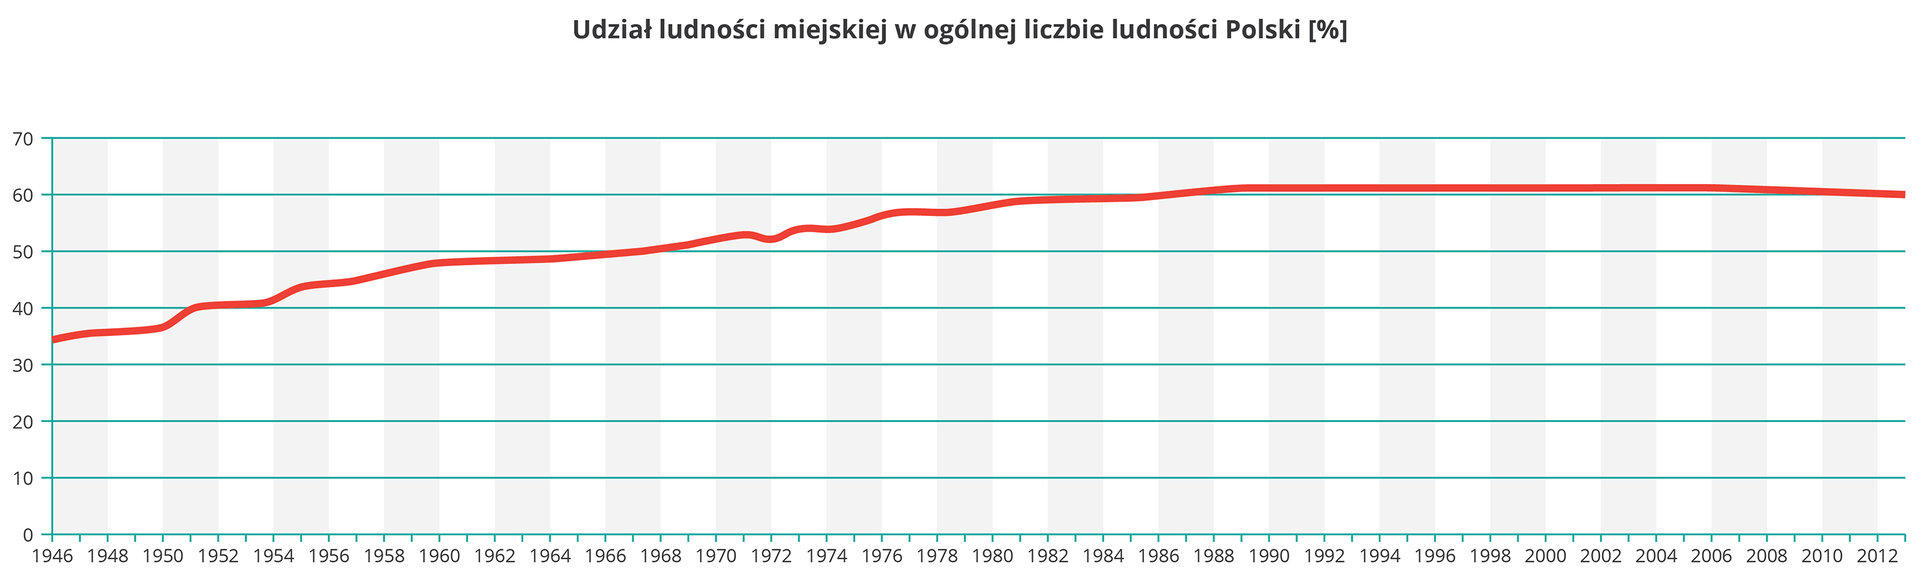
\includegraphics[width=0.8\textwidth]{urbanizacjawPolsce.png}
        \caption{Zescrapowany graf urbanizacji w Polsce}
\end{figure}
\subsection{Dane po obróbce}
Po wstępnej obróbce danych, tak prezentują się zmienne demograficzne po ich normalizacji:
\begin{figure}[H]
        \centering
        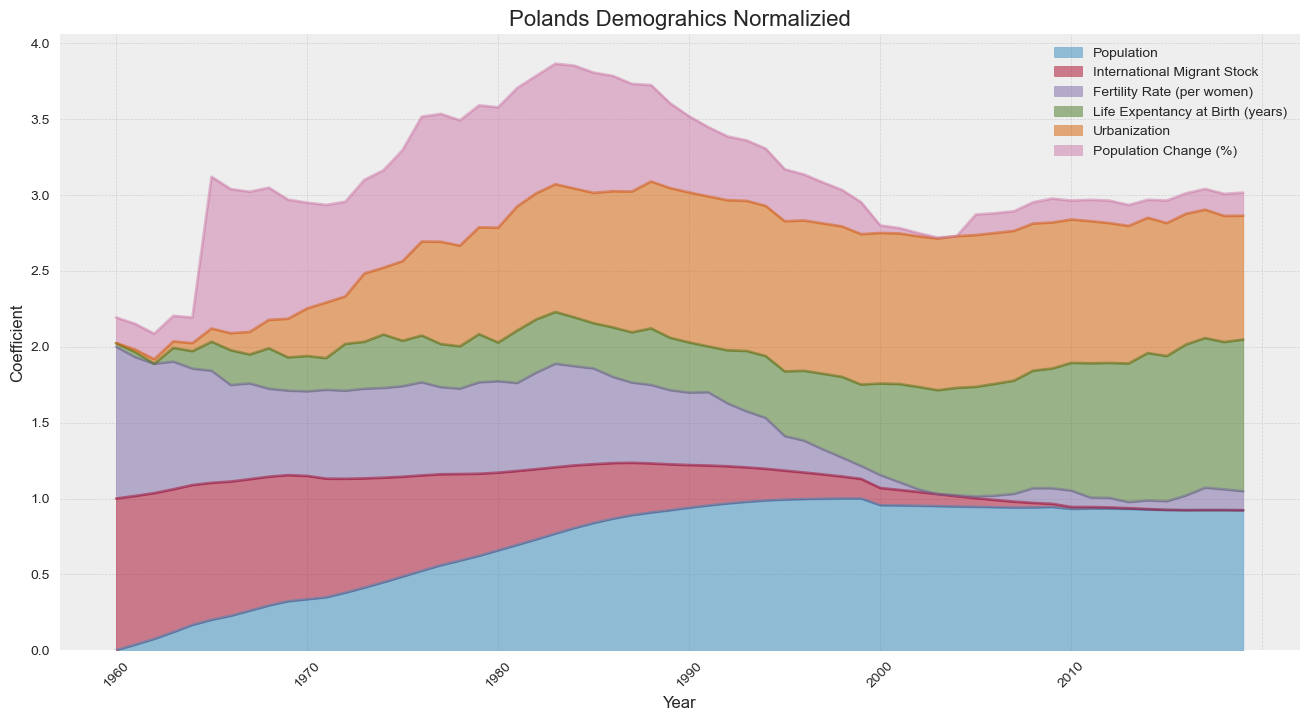
\includegraphics[width=0.8\textwidth]{images/normalized_all_vars.png}
        \caption{Dane po obróbce}
\end{figure}
\subsection{Analiza danych}
Do analizy eksploracyjnej danych wykorzystano bibliotekę pandas-profiling\cite{pp}
\subsection{Populacja w Polsce}
\begin{figure}[H]
        \centering
        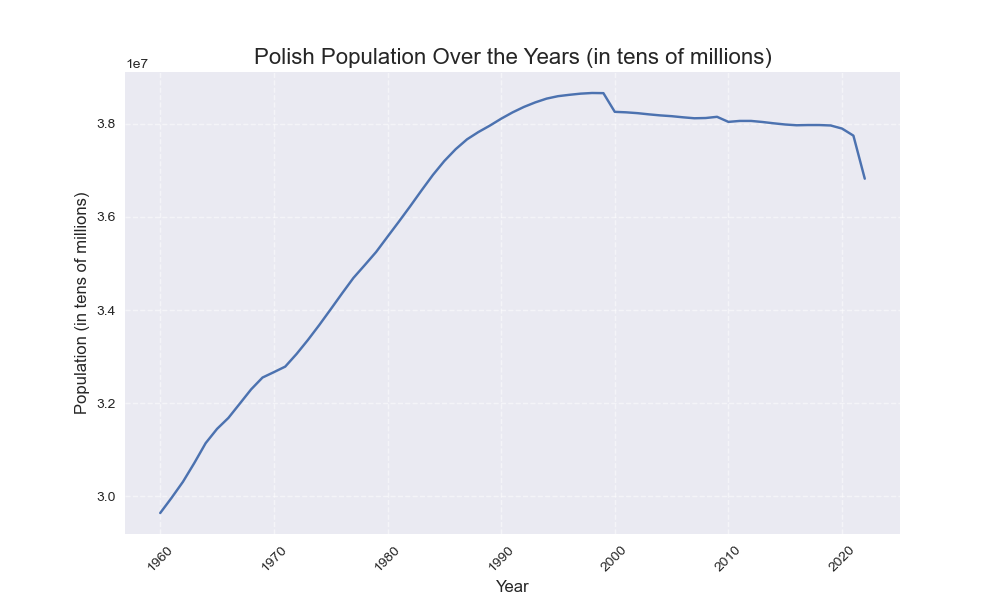
\includegraphics[width=0.8\textwidth]{polish_population_over_the_years.png}
        \caption{Wizualizacja liczby ludności w Polsce na przestrzeni lat}
\end{figure}
\begin{figure}[H]
        \centering
        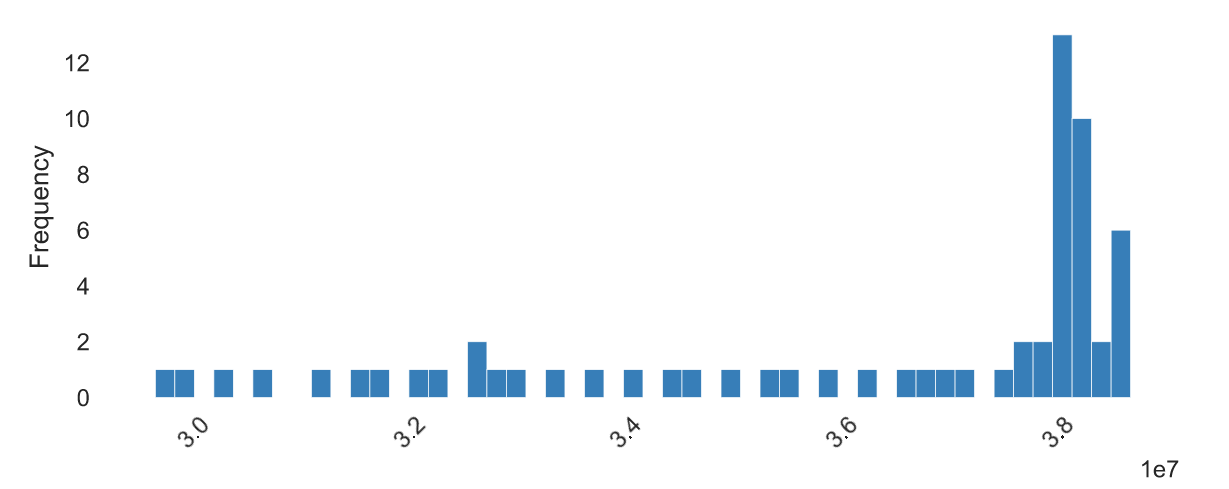
\includegraphics[width=0.8\textwidth]{images/histogram_populacja.png}
        \caption{Histogram liczby ludności w Polsce}
\end{figure}
\begin{table}[H]
        \centering
        \begin{tabular}{|l|l|l|}
        \hline
        Minimum & Maximum & Mediana \\ \hline
        29637450 & 38663481 & 37899070 \\ \hline
        \end{tabular}
        \caption{Statystyki liczby ludności w Polsce}
        \end{table}
\subsection{Imigracja do Polski}
\begin{figure}[H]
        \centering
        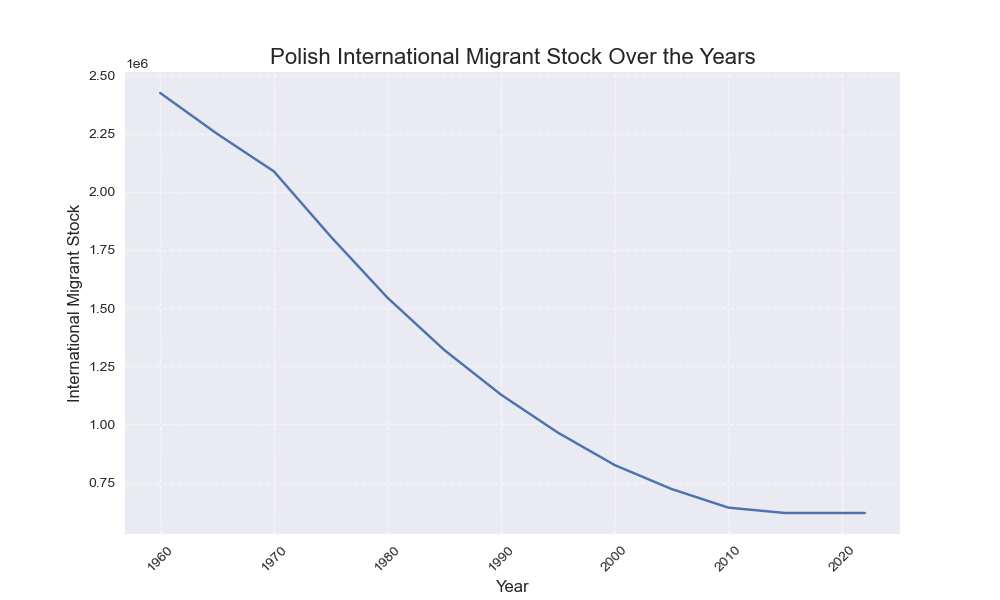
\includegraphics[width=0.8\textwidth]{polish_int_migrant_stock_over_the_years.png}
        \caption{Wizualizacja imigracji do Polski na przestrzeni lat}
\end{figure}
\begin{figure}[H]
        \centering
        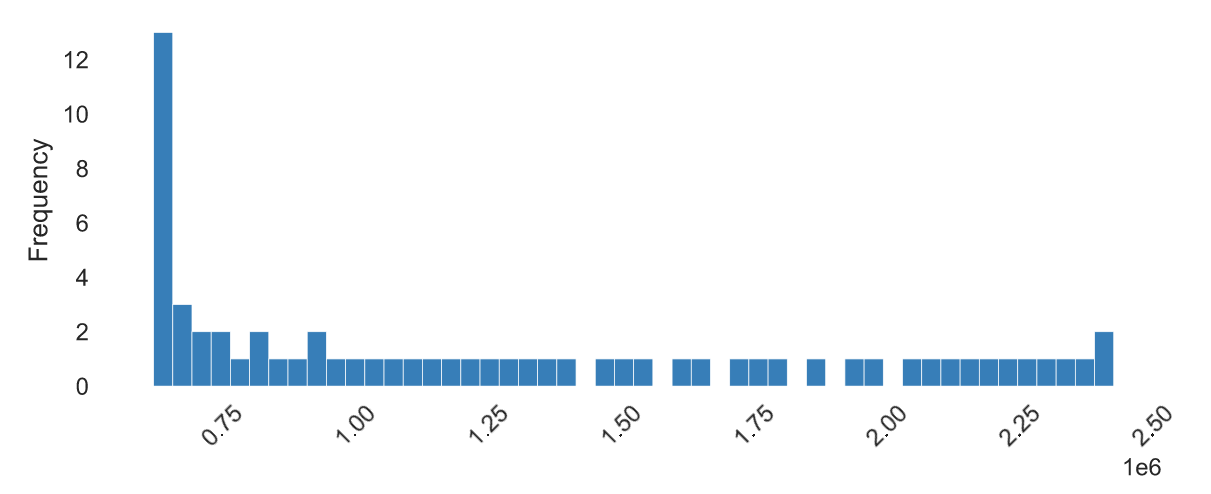
\includegraphics[width=0.8\textwidth]{images/histogram_imigracja.png}
        \caption{Histogram imigracji do Polski na przestrzeni lat}
\end{figure}
\begin{table}[H]
        \centering
        \begin{tabular}{|l|l|l|}
        \hline
        Minimum & Maximum & Mediana \\ \hline
        619403 & 2424881 & 1095161 \\ \hline
        \end{tabular}
        \caption{Statystyki imigracji do Polski}
        \end{table}
\subsection{Współczynnik dzietności}
\begin{figure}[H]
        \centering
        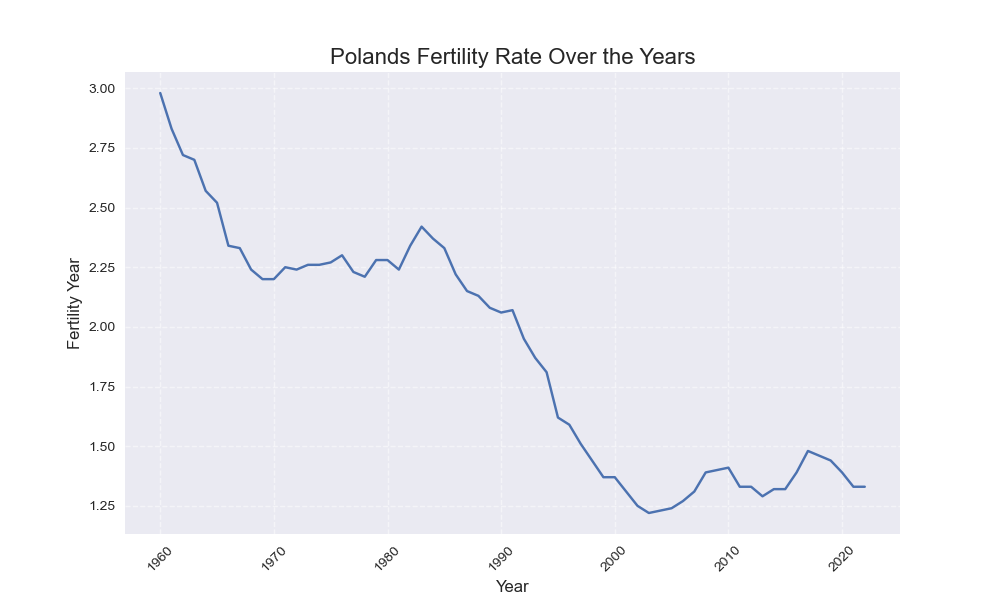
\includegraphics[width=0.8\textwidth]{polish_fertility_rate.png}
        \caption{Wizualizacja współczynnika dzietności Polski na przestrzeni lat}
\end{figure}
\begin{figure}[H]
        \centering
        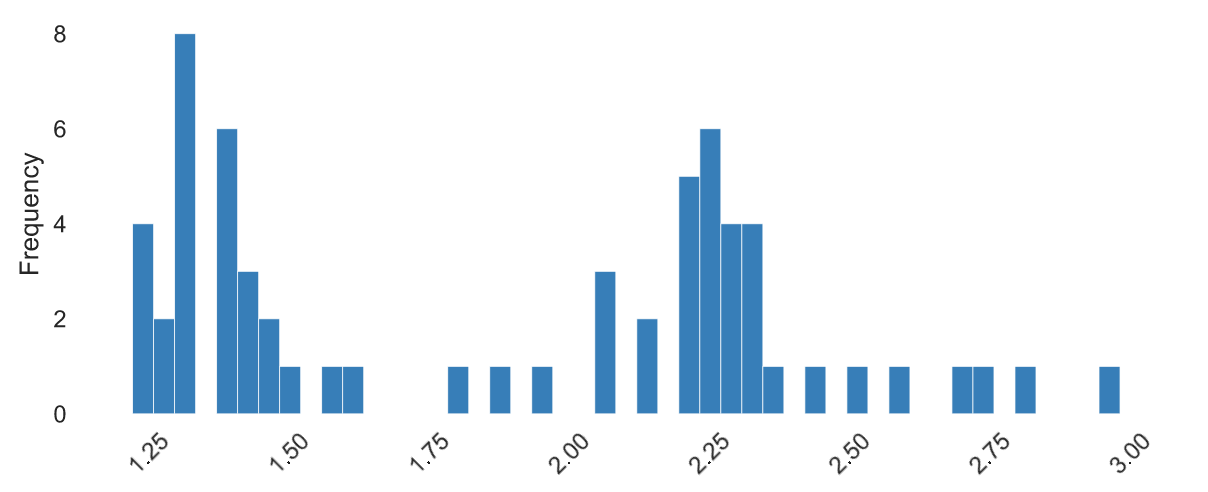
\includegraphics[width=0.8\textwidth]{images/histogram_dzietnosc.png}
        \caption{Histogram współczynnika dzietności na przestrzeni lat}
\end{figure}
\begin{table}[H]
        \centering
        \begin{tabular}{|l|l|l|}
        \hline
        Minimum & Maximum & Mediana \\ \hline
        1.22 & 2.98 & 2.06 \\ \hline
        \end{tabular}
        \caption{Statystyki współczynnika dzietności}
        \end{table}
\subsection{Oczekiwana długość życia}
\begin{figure}[H]
        \centering
        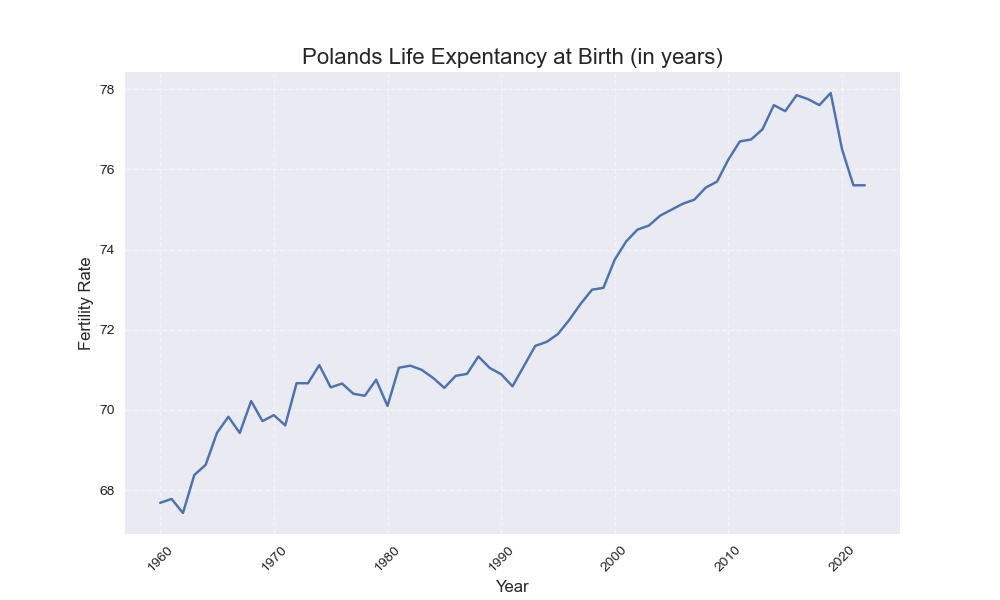
\includegraphics[width=0.8\textwidth]{polish_life_expentancy.png}
        \caption{Wizualizacja oczekiwanej długości życia na przestrzeni lat}
\end{figure}
\begin{figure}[H]
        \centering
        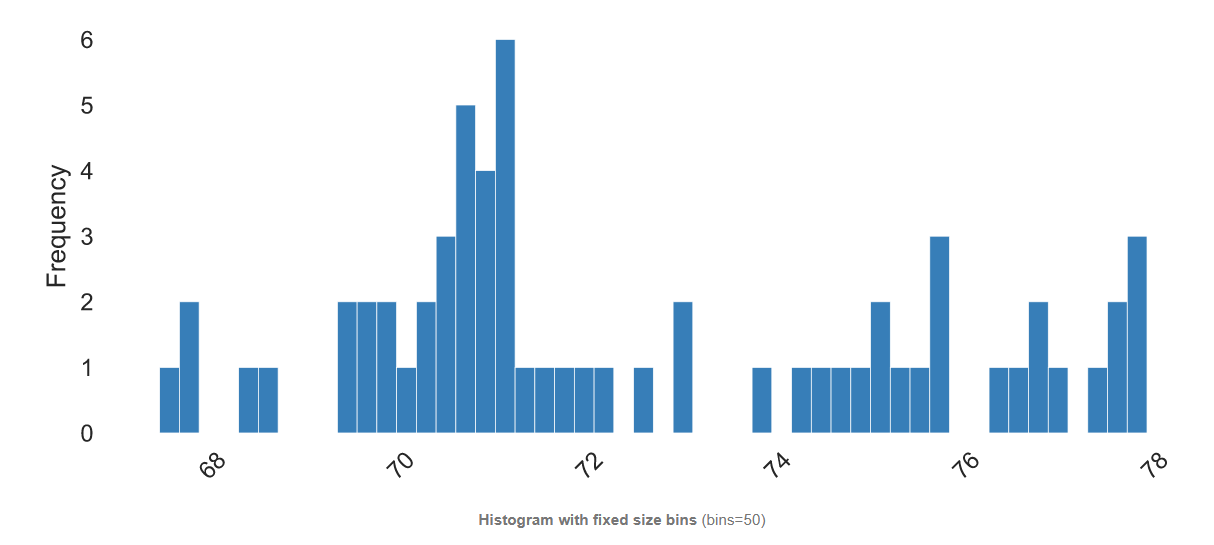
\includegraphics[width=0.8\textwidth]{images/histogram_dl_zycia.png}
        \caption{Histogram oczekiwanej długości życia na przestrzeni lat}
\end{figure}
\begin{table}[H]
        \centering
        \begin{tabular}{|l|l|l|}
        \hline
        Minimum & Maximum & Mediana \\ \hline
        67.42 & 77.9 & 71.1 \\ \hline
        \end{tabular}
        \caption{Statystyki oczekiwanej długości życia}
        \end{table}
\subsection{Urbanizacja}
\begin{figure}[H]
        \centering
        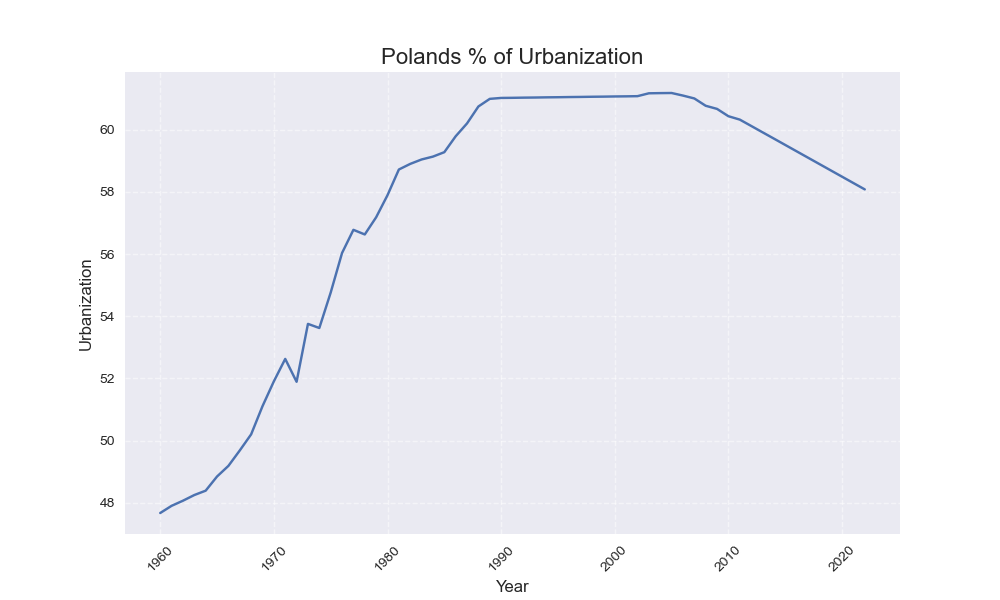
\includegraphics[width=0.8\textwidth]{polish_urbanization.png}
        \caption{Wizualizacja urbanizacji na przestrzeni lat}
\end{figure}
\begin{figure}[H]
        \centering
        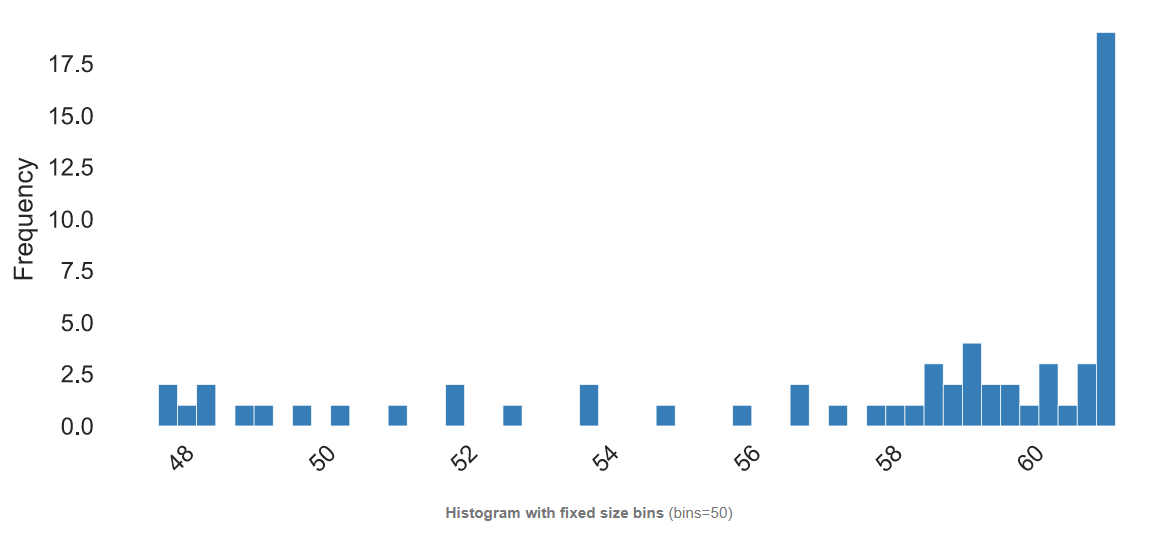
\includegraphics[width=0.8\textwidth]{images/histogram_urbanizacja.png}
        \caption{Wizualizacja urbanizacji na przestrzeni lat}
\end{figure}
\begin{table}[H]
        \centering
        \begin{tabular}{|l|l|l|}
        \hline
        Minimum & Maximum & Mediana \\ \hline
        47.66 & 61.18 & 59.27 \\ \hline
        \end{tabular}
        \caption{Statystyki urbanizacji}
        \end{table}
\subsection{Wskaźnik zmiany populacji}
\begin{figure}[H]
        \centering
        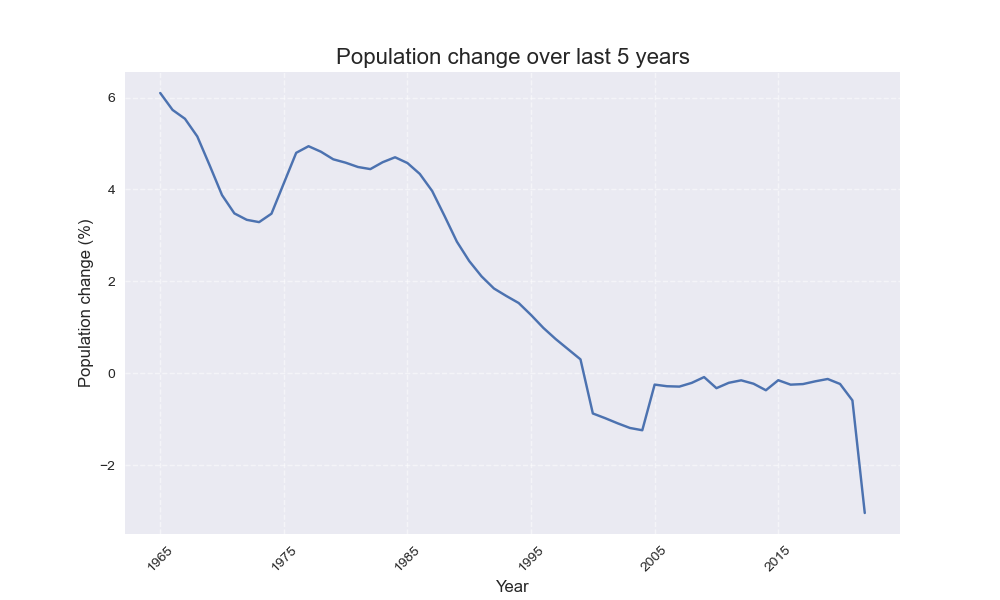
\includegraphics[width=0.8\textwidth]{polish_pop_change_5_years.png}
        \caption{Wizualizacja wskaźnika zmiany populacji na przestrzeni lat}
\end{figure}
\begin{figure}[H]
        \centering
        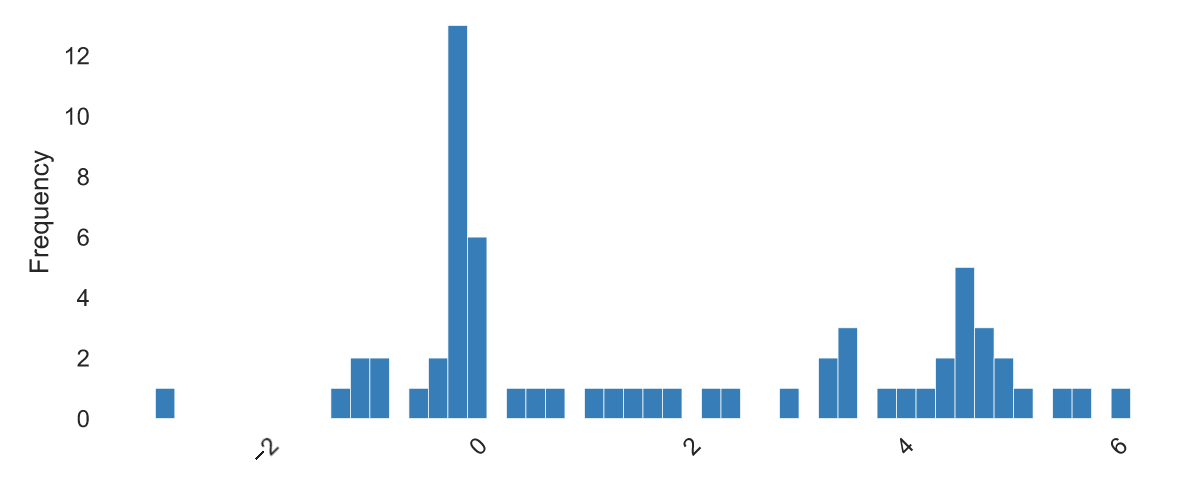
\includegraphics[width=0.8\textwidth]{images/histogram_zmiana_populacji.png}
        \caption{Histogram zmiany polskiej populacji na przestrzeni ostatnich 5 lat}
\end{figure}
\begin{table}[H]
        \centering
        \begin{tabular}{|l|l|l|}
        \hline
        Minimum & Maximum & Mediana \\ \hline
        -3.03 & 6.09 & 0.98 \\ \hline
        \end{tabular}
        \caption{Statystyki wskaźnika zmiany populacji}
        \end{table}
\subsection{Korelacja}
\begin{figure}[H]
        \centering
        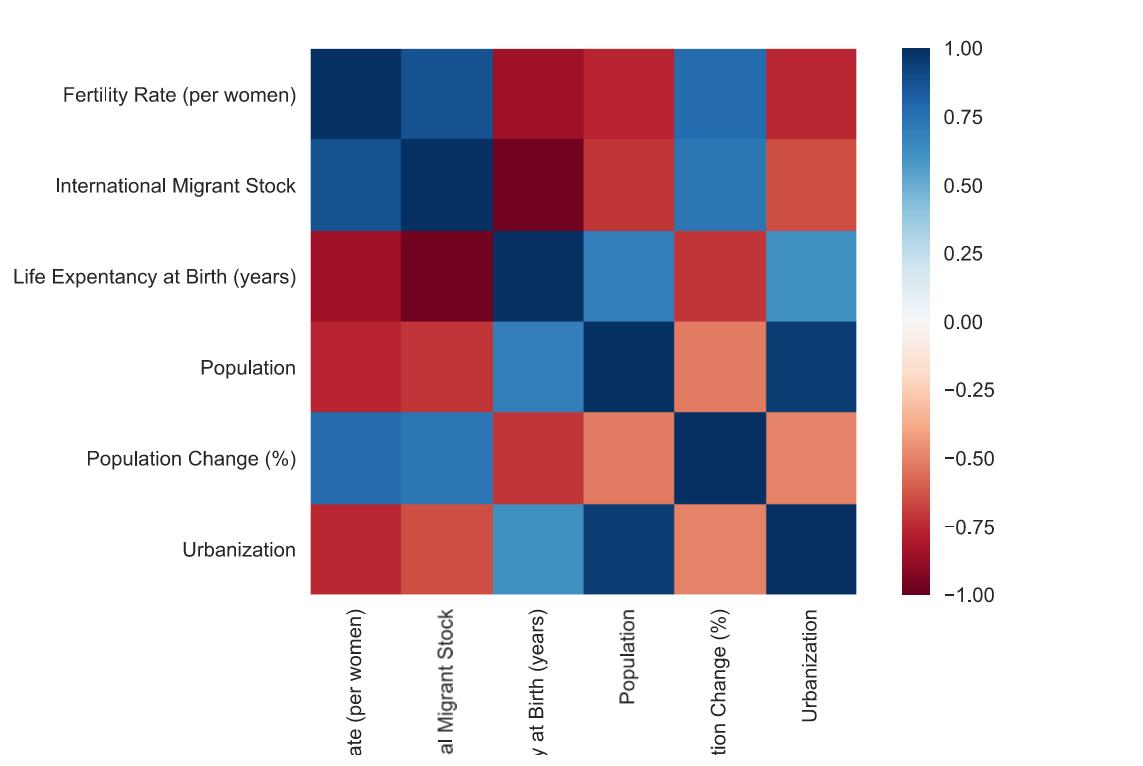
\includegraphics[width=0.8\textwidth]{images/matryca_korelacji.png}
        \caption{Macierz korelacji}
\end{figure}
        Z racji ręcznego dobioru danych i ich selekcji, analiza wykazała bardzo dużą korelację (oraz antykorelacje) pomiędzy wybranymi współczynnikami.
        Pojawia się bardzo zaskakująca, przecząca logice korelacja, pomiędzy współczynnikiem dzietności a populacją wynosząca -0.763.
        Prawdopodobnie wynika ona z tego że przez większość badanego okresu, współczynnik był nadal na bardzo wysokim poziomie, więc mimo że malał, to populacja stale się zwiększała.
        Analogicznie zaskakuje negatywna korelacja migracji z populacją, co także dziwi, ponieważ zgodnie z intuicją, imigracja powinna zwiększać populację.
        Prawdopodobnie wynika to z faktu, że dane dotyczące imigracji są niewielkie, co powoduje że słabo, choć wciąż, przekładają się na polską populację.
        Jeśli zaś chodzi o spodziewane korelacje, należy szczególnie zwrócić uwagę:
        \begin{itemize}
        \item Oczekiwana długość życia z populacją: 0.683
        \item Urbanizacja z populacją: 0.949
        \item Urbanizacja z oczekiwaną długością życia: 0.611
        \end{itemize}
        Korelacje te dobrze wróżą dla modeli regresji, ponieważ są one na tyle silne, że powinny pozwolić na skuteczne przewidywanie liczby ludności w Polsce.
\subsection{Eliminacja danych odstających}
Podczas przeglądania grafów reprezentujących zebrane dane, nie trudno było zauważyć że dane po 2019 roku są znacznie odstające od reszty.
Oczywistym jest że w 2020 roku, z racji pandemii, wiele wskaźników uległo zmianie, co sprawia że dane z tego roku są nieprzydatne do analizy.
Z tego powodu, dane z 2020 roku wzwyż zostały usunięte.
\section{Dobór metryk oceny}
Zanim przystąpimy do analizy modeli, należy zdefiniować metryki, które pozwolą nam ocenić ich skuteczność.
Dobór odpowiednich metryk jest kluczowy, ponieważ pozwala na obiektywną ocenę modeli, oraz porównanie ich ze sobą.
W przypadku regresji, najczęściej stosowanymi metrykami są:
\begin{itemize}
\item Mean Squared Error (MSE) - średni błąd kwadratowy
\item Mean Absolute Percentage Error (MAPE) - średni błąd procentowy bezwzględny
\item R2 Score - współczynnik determinacji
\end{itemize}
\subsection{Mean Squared Error}
MSE jest jedną z najczęściej stosowanych metryk w regresji. Oblicza ona średni błąd kwadratowy pomiędzy wartościami przewidywanymi przez model, a wartościami rzeczywistymi.
\begin{equation}
MSE = \frac{1}{n} \sum_{i=1}^{n} (y_i - \hat{y_i})^2
\end{equation}
\subsection{Mean Absolute Percentage Error}
MAPE jest metryką, która mierzy średni błąd procentowy bezwzględny pomiędzy wartościami przewidywanymi przez model, a wartościami rzeczywistymi.
\begin{equation}
MAPE = \frac{1}{n} \sum_{i=1}^{n} \frac{|y_i - \hat{y_i}|}{y_i}
\end{equation}
\subsection{R2 Score}
R2 Score jest metryką, która mierzy jak dobrze model przewiduje dane w porównaniu do średniej wartości. Wartość R2 Score może przyjmować wartości od $-\infty$
  do 1, gdzie 1 oznacza idealne dopasowanie modelu.
\begin{equation}
R2 = 1 - \frac{\sum_{i=1}^{n} (y_i - \hat{y_i})^2}{\sum_{i=1}^{n} (y_i - \bar{y})^2}
\end{equation}
\subsection{Analiza metryk}
Metryki zostały wybrane tak, aby pokrywały one różne aspekty oceny modeli. MSE pozwala na ocenę jak dobrze model przewiduje wartości, MAPE pozwala na ocenę jak dobrze model przewiduje wartości w procentach, a R2 Score pozwala na ocenę jak dobrze model przewiduje wartości w porównaniu do średniej wartości.
Nie ulega jednak wąptliwości że najlepszym wyborem jest MAPE, który najlepiej nadaje się do predykcji dotyczących populacji\cite{dop}, a więc jest najbardziej adekwatny do naszego problemu.
\section{Analiza modeli}
\subsection{Dla podziału 80/20}
Podział 80/20 oznacza to że model uczyć będzie się na danych z lat 1960-2008, a testowany będzie na danych z lat 2009-2019.
\subsubsection{Regresja liniowa}
\begin{figure}[H]
        \centering
        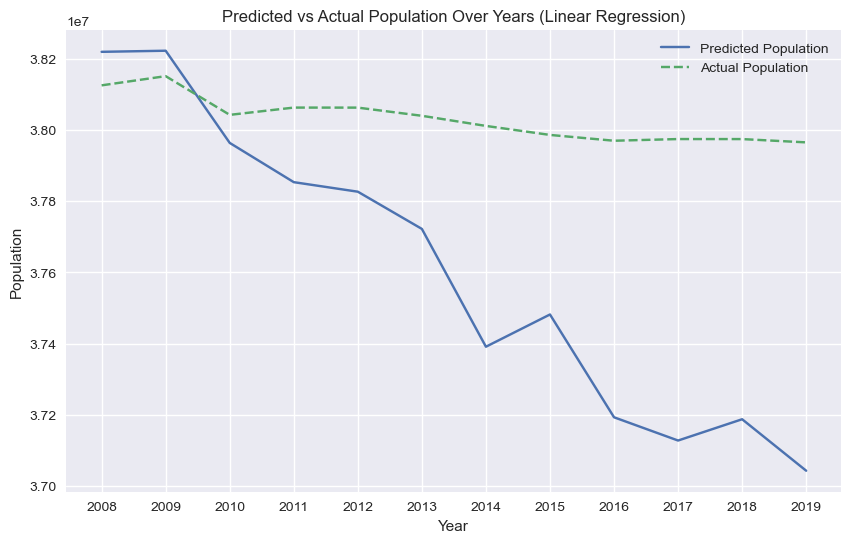
\includegraphics[width=0.8\textwidth]{images/linear.png}
        \caption{Regresja liniowa}
\end{figure}
\begin{table}[H]
        \centering
        \begin{tabular}{|l|l|l|l|}
        \hline
        Model & MSE & MAPE & R2 Score \\ \hline
        Linear Regression & 3.04e+11 & 0.012 & -84.972 \\ \hline
        \end{tabular}
        \caption{Metryki dla regresji liniowej i podziału 80/20}
        \end{table}
\subsubsection{Regresja Ridge}
\begin{figure}[H]
        \centering
        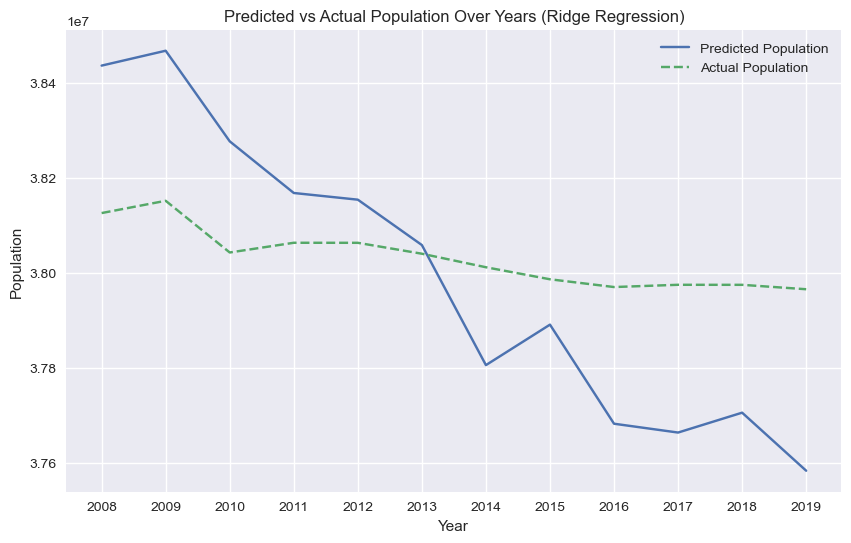
\includegraphics[width=0.8\textwidth]{images/ridge.png}
        \caption{Regresja Ridge}
\end{figure}
\begin{table}[H]
        \centering
        \begin{tabular}{|l|l|l|l|}
        \hline
        Model & MSE & MAPE & R2 Score \\ \hline
        Lasso Regression & 6.00e+10 & 0.006 & -15.926 \\ \hline
        \end{tabular}
        \caption{Metryki dla regresji Ridge i podziału 80/20}
        \end{table}
\subsubsection{Regresja Lasso}
\begin{figure}[H]
        \centering
        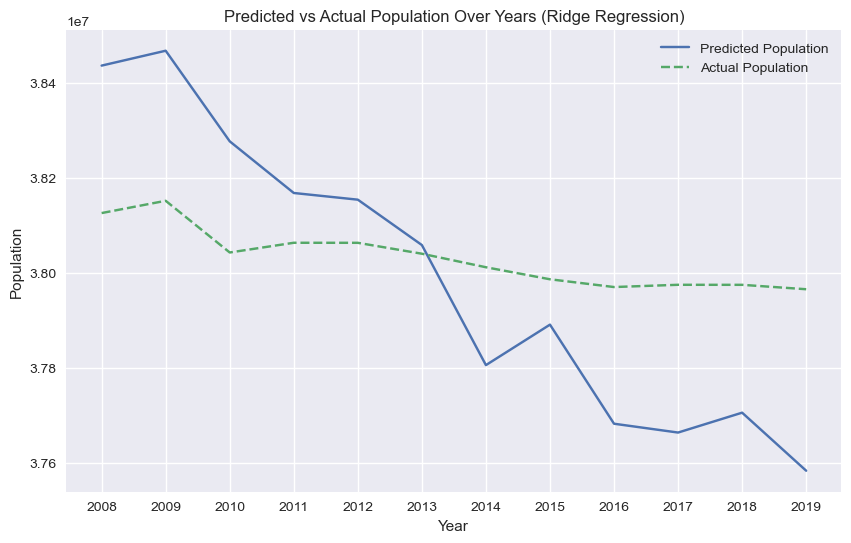
\includegraphics[width=0.8\textwidth]{images/lasso.png}
        \caption{Regresja Lasso}
\end{figure}
\begin{table}[H]
        \centering
        \begin{tabular}{|l|l|l|l|}
        \hline
        Model & MSE & MAPE & R2 Score \\ \hline
        Lasso Regression & 3.04e+11 & 0.011 & -84.952 \\ \hline
        \end{tabular}
        \caption{Metryki dla regresji Lasso i podziału 80/20}
        \end{table}
\subsubsection{Regresja Elastic Net}
\begin{figure}[H]
        \centering
        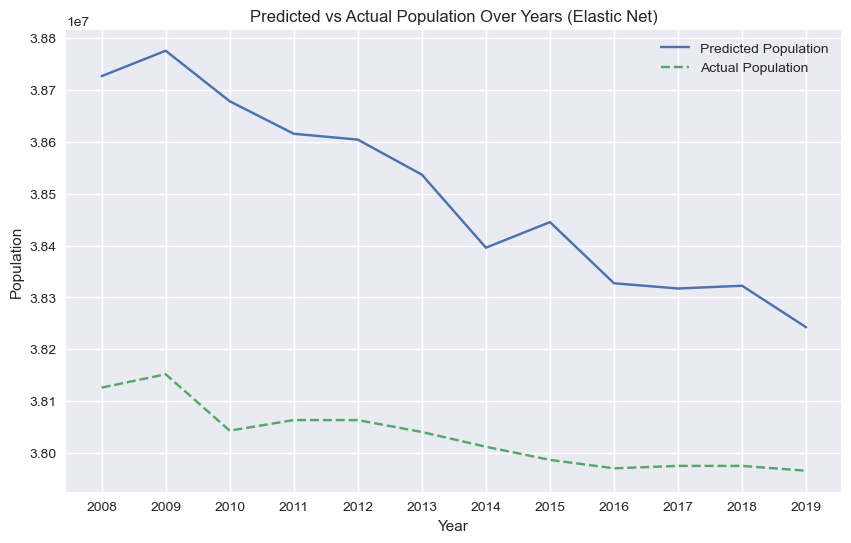
\includegraphics[width=0.8\textwidth]{images/elastic_net.png}
        \caption{Regresja Elastic Net}
\end{figure}
\begin{table}[H]
        \centering
        \begin{tabular}{|l|l|l|l|}
        \hline
        Model & MSE & MAPE & R2 Score \\ \hline
        Elastic Net & 2.33e+11 & 0.012 & -64.851 \\ \hline
        \end{tabular}
        \caption{Metryki dla regresji Elastic Net i podziału 80/20}
\end{table}
\subsubsection{Regresja Bayesian Ridge}
\begin{figure}[H]
        \centering
        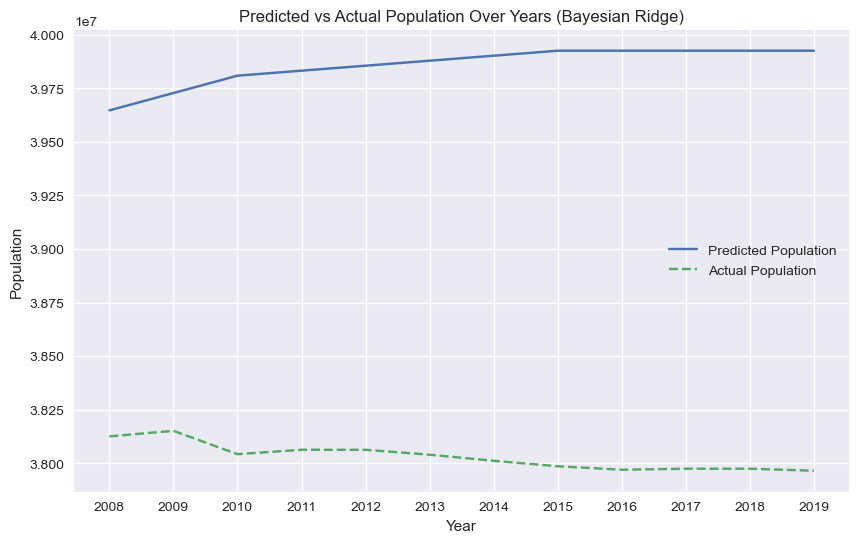
\includegraphics[width=0.8\textwidth]{images/bayesian_ridge.png}
        \caption{Regresja Bayesian Ridge}
\end{figure}
\begin{table}[H]
        \centering
        \begin{tabular}{|l|l|l|l|}
        \hline
        Model & MSE & MAPE & R2 Score \\ \hline
        Bayesian Ridge Regression & 3.35e+12 & 0.048 & -946.190 \\ \hline
        \end{tabular}
        \caption{Metryki dla regresji Bayesian Ridge i podziału 80/20}
        \end{table}
\subsubsection{Podsumowanie dla podziału 80/20}
\begin{table}[H]
        \centering
        \begin{tabular}{|l|l|l|l|}
        \hline
        Model & MSE & MAPE & R2 Score \\ \hline
        Linear Regression & 3.04e+11 & 0.012 & -84.972 \\ \hline
        Ridge Regression & 6.00e+10 & 0.006 & -15.926 \\ \hline
        Lasso Regression & 3.04e+11 & 0.011 & -84.952 \\ \hline
        Elastic Net & 2.33e+11 & 0.012 & -64.851 \\ \hline
        Bayesian Ridge & 3.35e+12 & 0.048 & -946.190 \\ \hline
        \end{tabular}
        \caption{Wyniki dla podziału 80/20}
\end{table}
Metryka MSE jest bardzo wysoka, co jest spowodowane tym że dane do przewidzenia są bardzo wysokie (rzędzu $10^7$), co sprawia że błędy są również bardzo wysokie.
Dodatkowo, model otrzymał niewielkie ilości danych szkoleniowych, co sprawia że jest on niewystarczająco dopasowany do danych testowych.
MAPE, która jest główną metryką, daje jednak nadzieje na to że model może być użyteczny, ponieważ wartość błędu procentowego dla Ridge wynosi zaledwie 0.006.
\begin{itemize}
        \item Najlepszym modelem okazała się regresja Ridge, która osiągnęła najniższe wartości MSE, MAPE oraz najwyższe R2 Score.
        \item Najgorszym modelem okazała się regresja Bayesian Ridge, która osiągnęła najwyższe wartości MSE, MAPE oraz niespotykanie niski R2 Score.
        \item Regresja Lasso oraz regresja liniowa osiągnęły bardzo zbliżone wyniki, co sprawia że nie można jednoznacznie stwierdzić która z nich jest lepsza.
        \item Regresja Elastic Net osiągnęła wyniki zbliżone, choć gorsze, od regresji Ridge, ale lepsze R2 i MSE niż Lasso i Liniowa, co sprawia że również jest ona dobrym modelem.
\end{itemize}
\subsection{Dla podziału 60/40}
Podział 60/40 oznacza to że model uczyć będzie się na danych z lat 1960-1995, a testowany będzie na danych z lat 1996-2019.
\subsubsection{Regresja liniowa}
\begin{figure}[H]
        \centering
        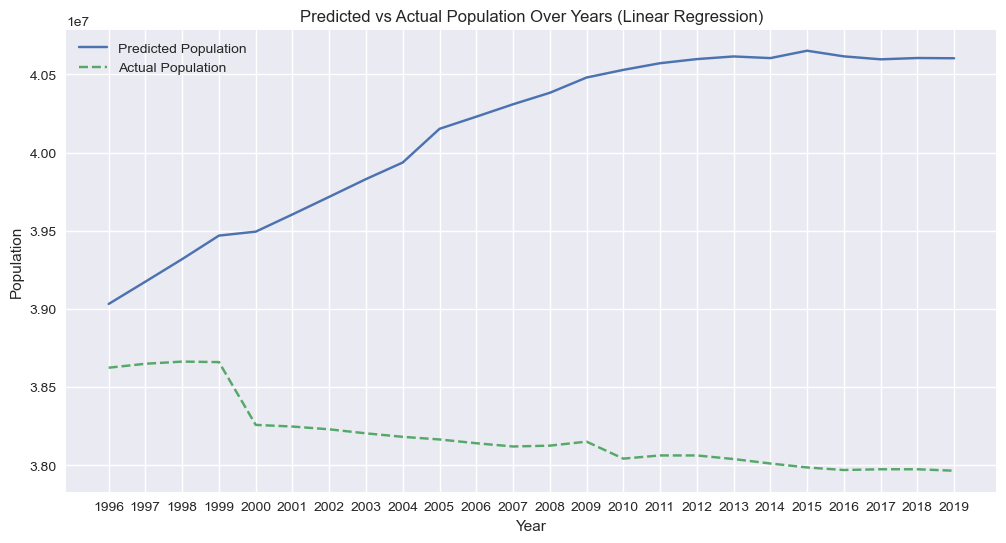
\includegraphics[width=0.8\textwidth]{images/linear996.png}
        \caption{Regresja liniowa}
\end{figure}
\begin{table}[H]
        \centering
        \begin{tabular}{|l|l|l|l|}
        \hline
        Model & MSE & MAPE & R2 Score \\ \hline
        Linear Regression & 4.31e+12 & 0.051 & -84.631 \\ \hline
        \end{tabular}
        \caption{Metryki dla regresji liniowej i podziału 60/40}
        \end{table}
\subsubsection{Regresja Ridge}
\begin{figure}[H]
        \centering
        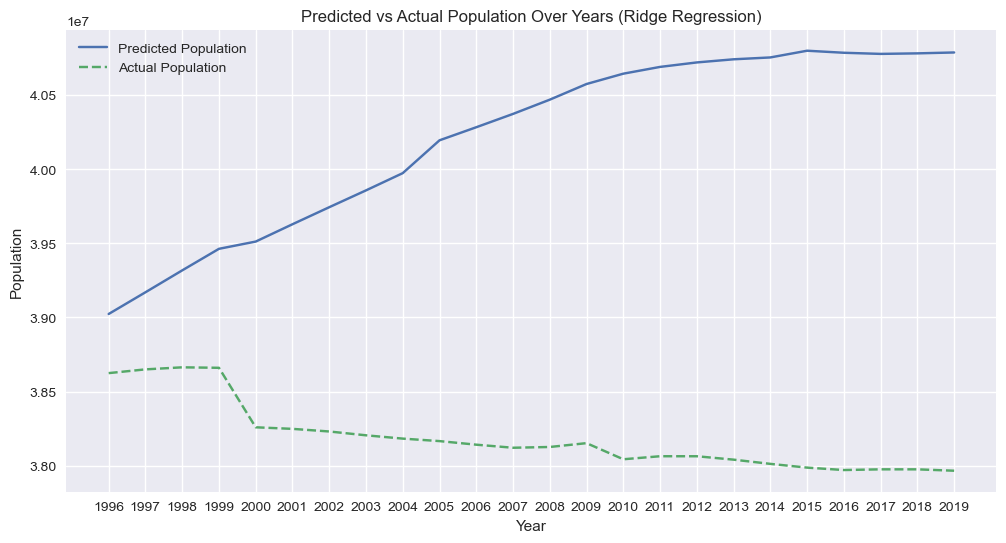
\includegraphics[width=0.8\textwidth]{images/ridge996.png}
        \caption{Regresja Ridge}
\end{figure}
\begin{table}[H]
        \centering
        \begin{tabular}{|l|l|l|l|}
        \hline
        Model & MSE & MAPE & R2 Score \\ \hline
        Ridge Regression & 4.73e+12 & 0.053 & -92.887 \\ \hline
        \end{tabular}
        \caption{Metryki dla regresji Ridge i podziału 60/40}
        \end{table}
\subsubsection{Regresja Lasso}
\begin{figure}[H]
        \centering
        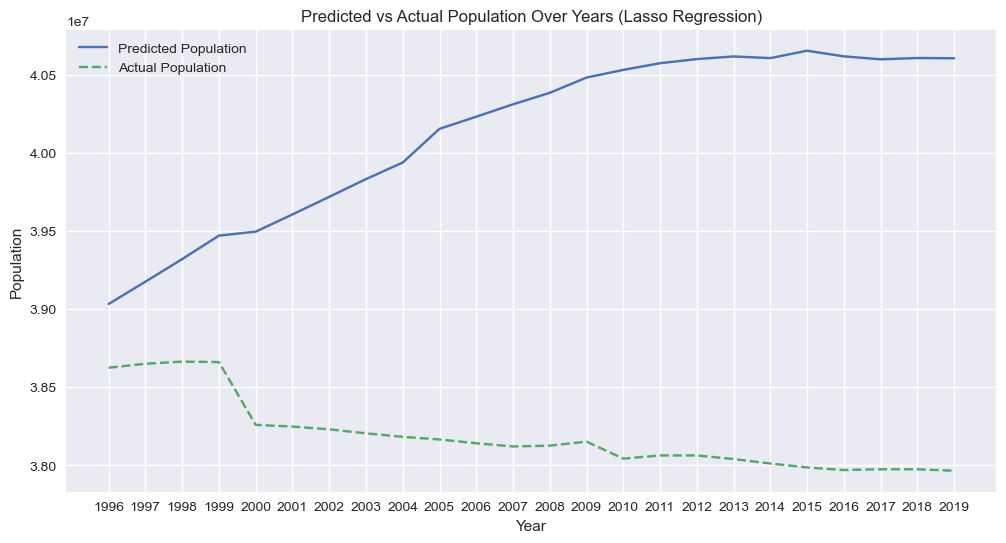
\includegraphics[width=0.8\textwidth]{images/lasso996.png}
        \caption{Regresja Lasso}
\end{figure}
\begin{table}[H]
        \centering
        \begin{tabular}{|l|l|l|l|}
        \hline
        Model & MSE & MAPE & R2 Score \\ \hline
        Lasso Regression & 4.31e+12 & 0.050 & -84.638 \\ \hline
        \end{tabular}
        \caption{Metryki dla regresji Lasso i podziału 60/40}
\end{table}
\subsubsection{Regresja Elastic Net}
\begin{figure}[H]
        \centering
        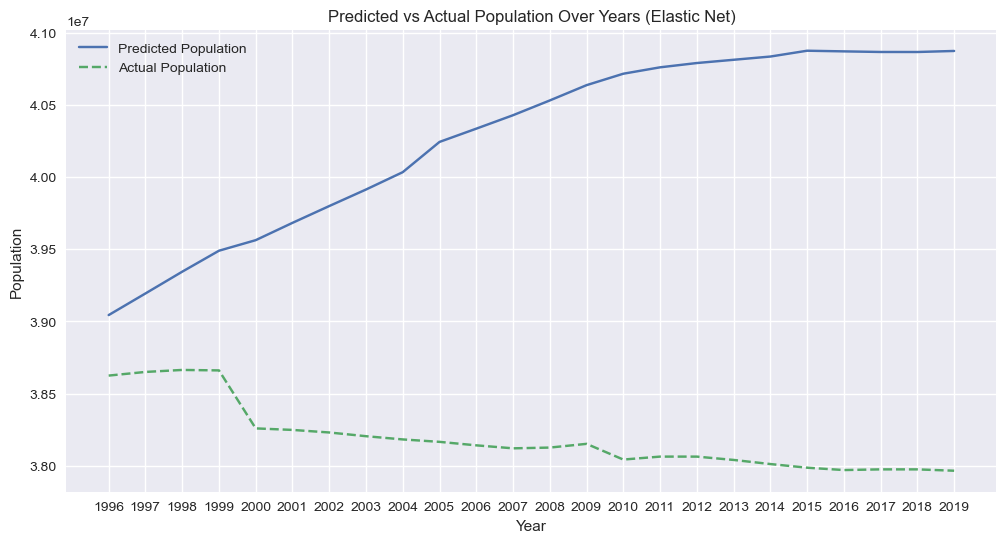
\includegraphics[width=0.8\textwidth]{images/elastic_net996.png}
        \caption{Regresja Elastic Net}
\end{figure}
\begin{table}[H]
        \centering
        \begin{tabular}{|l|l|l|l|}
        \hline
        Model & MSE & MAPE & R2 Score \\ \hline
        Elastic Net & 4.99e+12 & 0.054 & -98.200 \\ \hline
        \end{tabular}
        \caption{Metryki dla regresji Elastic Net i podziału 60/40}
\end{table}
\subsubsection{Regresja Bayesian Ridge}
\begin{figure}[H]
        \centering
        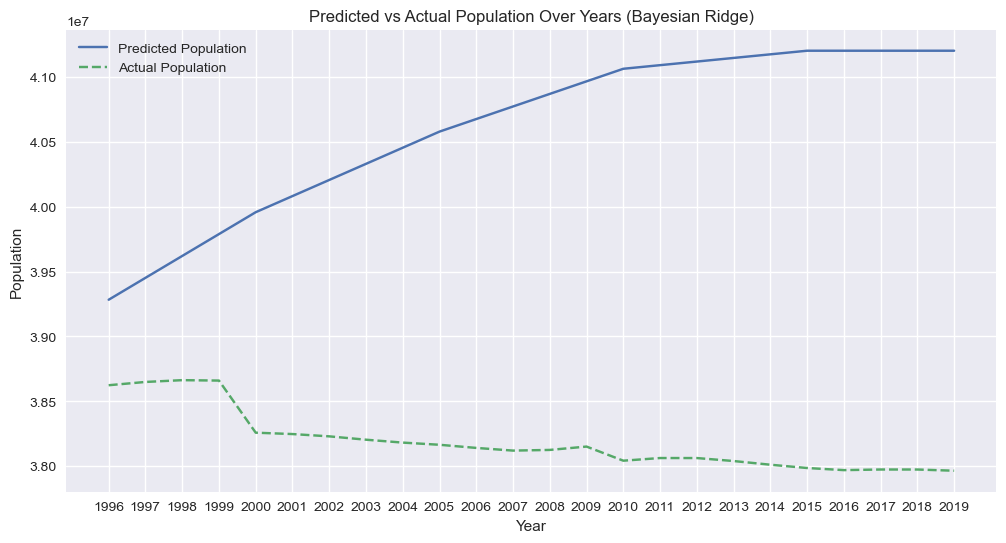
\includegraphics[width=0.8\textwidth]{images/bayesian_ridge996.png}
        \caption{Regresja Bayesian Ridge}
\end{figure}
\begin{table}[H]
        \centering
        \begin{tabular}{|l|l|l|l|}
        \hline
        Model & MSE & MAPE & R2 Score \\ \hline
        Bayesian Ridge & 6.55e+12 & 0.063 & -129.007 \\ \hline
        \end{tabular}
        \caption{Metryki dla regresji Bayesian Ridge i podziału 60/40}
\end{table}
\subsubsection{Podsumowanie dla podziału 60/40}
\begin{table}[H]
        \centering
        \begin{tabular}{|l|l|l|l|}
        \hline
        Model & MSE & MAPE & R2 Score \\ \hline
        Linear Regression & 4.31e+12 & 0.051 & -84.631 \\ \hline
        Ridge Regression & 4.73e+12 & 0.053 & -92.887 \\ \hline
        Lasso Regression & 4.31e+12 & 0.050 & -84.638 \\ \hline
        Elastic Net & 4.99e+12 & 0.054 & -98.200 \\ \hline
        Bayesian Ridge & 6.55e+12 & 0.063 & -129.007 \\ \hline
        \end{tabular}
        \caption{Wyniki dla podziału 60/40}
        \end{table}
Jak widać, wyniki dla podziału 60/40 są znacznie gorsze niż dla podziału 80/20. Wynika to z faktu że model otrzymał mniej danych szkoleniowych, co sprawia że jest on niewystarczająco dopasowany do danych testowych.
Split 80/20 okazał się zdecydowanie lepszy, co sprawia że jest on bardziej odpowiedni do analizy, i zapewnia dobry bilans między szkoleniem i testowaniem modelu.
\section{Wnioski}
Po przeanalizowaniu wielu różnych modeli regresji, na róznych podziałach danych, można stwierdzić że regresja Ridge jest najlepszym modelem do przewidywania liczby ludności w Polsce.
Model ten osiągnął najniższe wartości MSE, MAPE oraz najwyższe R2 Score, co sprawia że jest on najbardziej adekwatny do naszego problemu.
Warto szczególnie zwrócić uwagę na wartoścć MAPE, która wynosi zaledwie 0.006, co oznacza że model przewiduje wartości zaledwie o 0.6\% odchylające się od wartości rzeczywistych.
Kategoryzuje to ten model w kategorię bardzo dobrych\cite{rg}, co sprawia że jest on najbardziej odpowiedni do przewidywania liczby ludności w Polsce.\par
Dodatkowo, projekt ten udowania że zmienne demograficzne, takie jak dzietność, oczekiwana długość życia, urbanizacja, oraz imigracja, mają duży wpływ na liczebność populacji,
do tego stopnia, że na ich podstawie można z dużą dokładnością przewidzieć liczebność populacji w przyszłości.
Oczywiście, jak pokazał przykład pandemii COVID-19, zdarzenia losowe mogą znacząco wpłynąć na liczebność populacji, co sprawia że model ten nie jest idealny, ale nadal jest on bardzo dobrym narzędziem do przewidywania liczby ludności w Polsce,
i może być użyty do analizy trendów demograficznych w przyszłości, zwłaszcza w sytuacjach stablilnych, gdzie nie występują znaczące zmiany w populacji.\par
Ciekawą i wartą uwagi obserwacją, bez wątpienia jest fakt, że najlepsze modele regresji liniowej, przewidywały populację niższą niż rzeczywista.
W istocie może być to wytłumaczone faktem, że dane imigracyjne mogły być zaniżone, co przełożyło się na fakt że modele przewidywały zaniżoną populację.
\bibliographystyle{plain}
\bibliography{bibliografia}
\end{document}
